\section*{Week 5: Solution for selecting final set of keywords}
\addcontentsline{toc}{section}{Week 5: Solution for selecting final set of keywords}

Continuing from last week: With respect to each STRIDE cateogry, when referencing the list keywords we just obtained, eg. \textit{S\_final}, and the initial list of keywords we obtained, there exists an underlying problem where we are unsure of which words should be deleted or kept for training the model.\\
The solution I implemented using \textit{word2vec} to compare both lists and compare the similarities between words and set a minimum cosine value threshold. Any words with similarities below the threshold are deemed 'not similar enough' and will be dropped. \\
Through experimentation, the threshold value selected is 0.28. An example can be found in \hyperref[subsec:appendix2]{Appendix 2}\\

\begin{lstlisting}[frame=single]
def merge_lists(l1, min_cosine_value, w2v, ref_list):
final_list = []

for word in l1:
    if word in w2v:
        similarities = []
        for ref_word in ref_list:
            if ref_word in w2v:
                sim = w2v.similarity(word, ref_word)
                similarities.append(sim)
        if any(sim >= min_cosine_value for sim in similarities):
            final_list.append(word)
if 'use' in final_list: final_list.remove('use')
elif 'also' in final_list: final_list.remove('also')
return final_list
\end{lstlisting}

\begin{table}[h]
    \caption{Comparing keywords (arbitary example)}
    \label{crouch}
    \begin{tabularx}{\textwidth}{p{0.3\textwidth}XX}
        \toprule
        \textbf{Original set} & \textbf{Manually filtered set} & \textbf{Resultant set + words removed by semantic analysis} \\
        \midrule
        domain, activity, high, direct, include, path, relationship, network, gather, visibility, software, potentially, difficult, make, trusted, supply, gathering, manage, access, form, via, compromise, place, accounts, business, information, focus, elicitation, lifecycle, drive, defender, second, effort, set, provider, take, victim, social, owned, outside, phishing, operational, positive, reconnaissance, stage, domains, party, associate, way, false, variety, chain, well, connect, service, hardware, opportunity, various, online, organization, detection, search, accessible, this, media, target, use, elevate, detail, initial, data, adversary, related, reveal, occurrence, establish, third, etc, expose, relationships, resource, shipment, contractor, ex, open, rate, websites, also
        &
        authenticate, username, password, access, information, detection, take, include, malicious, control, network, search, name, access, infrastructure, traffic, data, suspicious, trust, reconnaissance, email, phishing, resource, initial, visibility, monitor, server, form, open, potentially, websites, address, process, detect, credential, file, certificate, internet, install, key, online, link, source
        &
        domain, include, relationship, network, gather, visibility, software, potentially, make, trusted, manage, access, form, via, information, lifecycle, provider, take, phishing, operational, reconnaissance, domains, connect, service, hardware, online, organization, detection, search, accessible, media, use, initial, data, reveal, establish, expose, relationships, resource, open, websites, \sout{source, file, malicious, certificate, monitor, authenticate, suspicious, email, install, server, link, detect, control, trust, address, credential, internet, process, password, traffic, key, username, name, infrastructure} \\
        \bottomrule
    \end{tabularx}
\end{table}
\clearpage

A word cloud for each STRIDE category is generated to visualise the keywords.
\begin{figure}[h]
    \centering
    \begin{subfigure}{0.45\textwidth}
        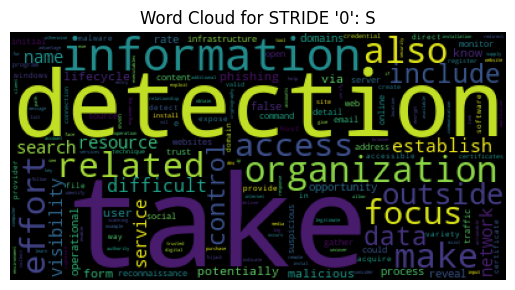
\includegraphics[width=\linewidth]{wordcloud/wc_0S.png}
    \end{subfigure}
    \hfill
    \begin{subfigure}{0.45\textwidth}
        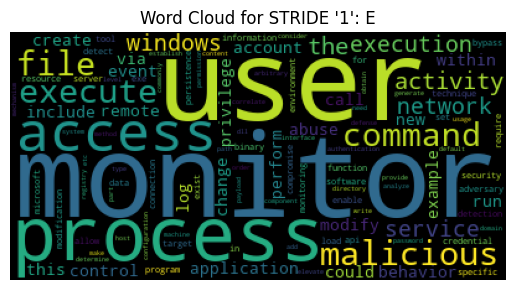
\includegraphics[width=\linewidth]{wordcloud/wc_1E.png}
    \end{subfigure}
    
    \medskip
    
    \begin{subfigure}{0.45\textwidth}
        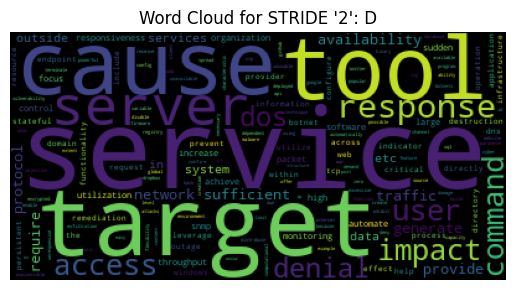
\includegraphics[width=\linewidth]{wordcloud/wc_2D.png}
    \end{subfigure}
    \hfill
    \begin{subfigure}{0.45\textwidth}
        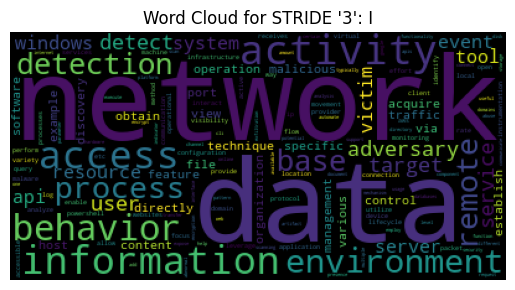
\includegraphics[width=\linewidth]{wordcloud/wc_3I.png}
    \end{subfigure}
    
    \medskip
    
    \begin{subfigure}{0.45\textwidth}
        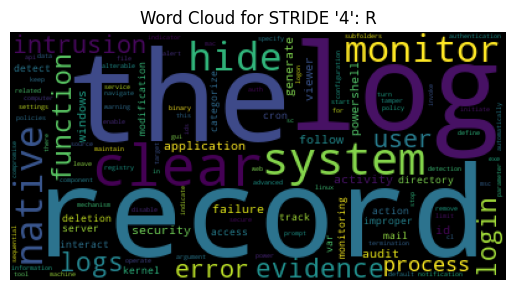
\includegraphics[width=\linewidth]{wordcloud/wc_4R.png}
    \end{subfigure}
    \hfill
    \begin{subfigure}{0.45\textwidth}
        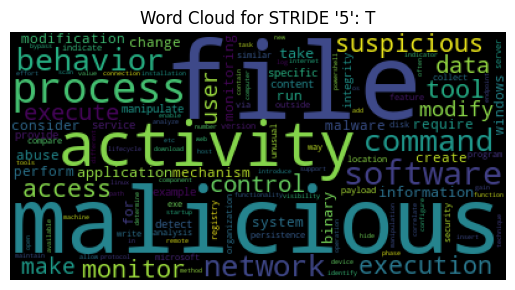
\includegraphics[width=\linewidth]{wordcloud/wc_5T.png}
    \end{subfigure}
    \label{fig:grid}
\end{figure}

Moving on, using the right most column of Table 5, I tokenize them and pass it into a multi-layer perceptron model where it is fine-tuned by hyperparamter testing (\hyperref[subsec:appendix3]{Appendix 3}). \\
\begin{lstlisting}[frame=single]
hidden_units = 128
batch_size = 16
num_epochs = 50
num_classes = 6
classes = [0,1,2,3,4,5]
vocab_size = X_train_tfidf.shape[1]
optimizer = tf.keras.optimizers.legacy.Adam(1e-4)

model5 = tf.keras.Sequential([
    tf.keras.layers.Input(shape=(vocab_size,)),
    tf.keras.layers.Dense(hidden_units*2, activation='leaky_relu'),
    tf.keras.layers.Dropout(.2),
    tf.keras.layers.BatchNormalization(),
    tf.keras.layers.Dense(hidden_units, activation='leaky_relu'),
    tf.keras.layers.Dropout(.2),
    tf.keras.layers.BatchNormalization(),
    tf.keras.layers.Dense(hidden_units//2, activation='leaky_relu'),
    tf.keras.layers.Dense(num_classes, kernel_regularizer=tf.keras.regularizers.L2(l2=1e-3), activation='softmax')
])

model5.compile(optimizer=optimizer, loss="sparse_categorical_crossentropy", metrics=['accuracy'])
model5.summary()
\end{lstlisting}

The results of this model is as follows:\\
\includegraphics*[scale=0.528]{cmatrix_model5.png}

This model seems to perform terribly on 'T' and 'E' categories.

Some improvements to be done:
\begin{itemize}[topsep=0pt]
    \item Create a separate model to classify 'T' and 'E' as they yield low accuracies. Then try to combine these models with \textit{model5}
    \item Evaluate the usefulness of \textit{LLaMA} model
\end{itemize}